%!TEX root = ../main.tex
\section{Networking}
The system deviced throughout this report seeks to ease the task of collecting data from the go-kart.
This is done by creating a network on the go-kart which allows the user to more easily add additional sensors.
In addition to providing a flexible platform for adding sensors, it will collect the data produced by the sensors on the network.
A goal with the project is to be able to monitor relevant data live through some interface.
To properly monitor data collected during driving it is necessary to maintain a live feed from the go-kart to the observer.
\\~\\
As mentioned above, there are two major functions to the system; recording of data and monitoring of data.
The recording is done on the go-kart using embedded hardware, specifically the Zybo platform is used to interface to the sensors.
The monitoring is done using a PC.
Monitoring is less time critical than the recording as it is simply meant for human readability.
For this reason, and to ease the workload, it has been decided to use a wifi connection between the go-kart and the PC.
Wifi, or even TCP/IP over ethernet is not viable on the go-kart between the Zybo boards due to the potentially long lag in that protocol.
A different network type will have to be devised for the embedded portion of the system.
This splits the network up into two parts, one that links the PC to the go-kart and one that links each component on the go-kart.
See figure \ref{fig:basic_network}.

\begin{figure}
	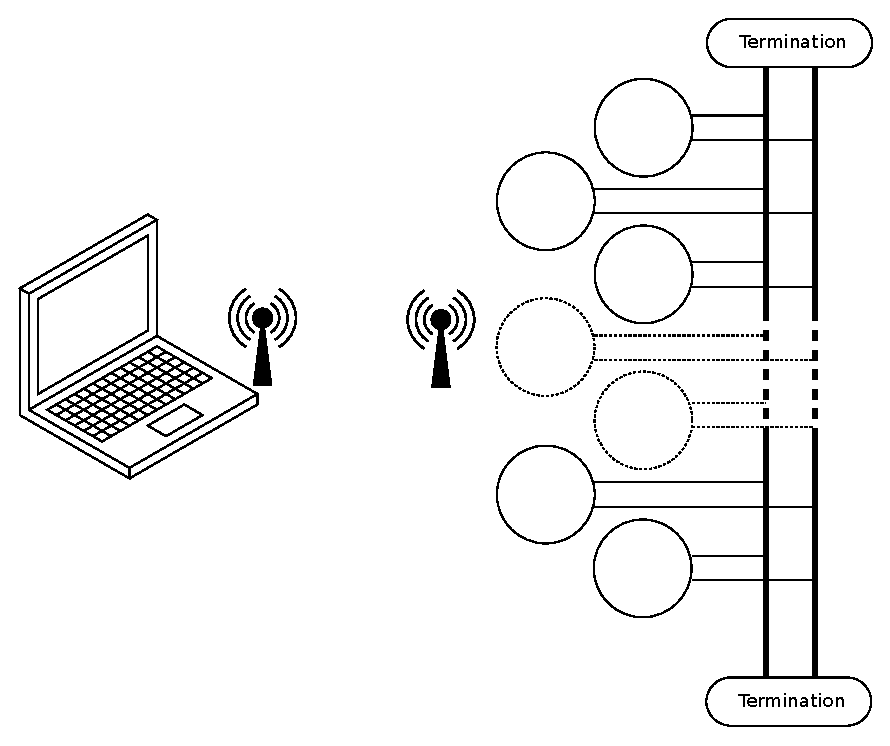
\includegraphics[width=.75\linewidth]{graphics/basic_network}
	\caption{A line of text}
	\label{fig:basic_network}
\end{figure}

These will be referred to as the off-kart network and the on-kart network, respectively, throughout the remainder of the report.
The following sections will explore the creation of both of these networks in turn.

\subsection{Off-Kart Network}
As mentioned above, the off-kart network is done using wifi.
It was chosen to use this method as all modern laptops are equipped with the capability of connecting to such a network.
Hereafter the challenge lies in establishing an ad-hoc network between a zybo board and a PC.
This network is created using the a USB-Wifi dongle on the Zybo board. 
The following script is run to bring down the device, change the network type to ad-hoc, bring up the device, create the ad-hoc network and, finally, assign an IP-address to the device.
\begin{lstlisting}
sudo ip link set wlan0 down
sudo iw wlan0 set type ibss
sudo ip link set wlan0 up
sudo iw wlan0 ibss join go-kart 2412
sudo ifconfig wlan0 192.168.10.9
\end{lstlisting}
It is verified working using the ping command from both the Zybo board and to the PC and vice versa.
Below is a thorough description of the challenges encountered while setting up this device as well as a brief explanation of the choice of device.
\\~\\
Two methods were immediately available for use: A usb wifi dongle and a PMOD wifi interface.
As the name implies, the latter is designed to be compatible with the PMOD interfaces on the zybo board (and a range of similar boards offered by Digilent Inc.).
It converts TCP/IP to SPI and vice versa.
However, since the zybo boards are already running a linux distribution, it was decided to attempt connecting through the usb wifi dongle.
This decision marked the beginning of a long journey, the highlights of which are discussed below. 
\\~\\
The first step was to ensure that the correct drivers are present on the system.
The usb dongle is a TP-LINK TL-WN722N.
This device uses the Atheros AR9271 chipset and is on the list of supported devices for the ath9k\_htc driver on wireless.wiki.kernel.org.
Running \texttt{dmesg} prints the kernel log, revealing, amongst other things, what drivers are loaded.
\begin{lstlisting}
dmesg | grep ath
[10.329564] usb 1-1: ath9k_htc: Firmware htc_9271.fw requested
[10.332438] usbcore: registered new interface driver ath9k_htc
\end{lstlisting}
Additionally:
\begin{lstlisting}
lsusb | grep Ath
Bus 001 Device 002: ID 0cf3:9271 Atheros Communications, 
	Inc. AR9271 802.11n
\end{lstlisting}
As per these commands the operating system (OS) has correctly detected and loaded the driver.
The \texttt{iproute2} package contains the utilities used to manipulate TCP/IP connections.
\begin{lstlisting}
ip link show
1: lo: <LOOPBACK,UP,LOWER_UP> mtu 65536 qdisc noqueue 
	state UNKNOWN mode DEFAULT group default 
    link/loopback 00:00:00:00:00:00 brd 00:00:00:00:00:00
2: eth0: <BROADCAST,MULTICAST,UP,LOWER_UP> mtu 1500 qdisc pfifo_fast 
	state UP mode DEFAULT group default qlen 1000
    link/ether 00:0a:35:00:01:22 brd ff:ff:ff:ff:ff:ff
3: wlan0: <BROADCAST,MULTICAST> mtu 1500 qdisc mq 
	state DOWN mode DEFAULT group default qlen 1000
    link/ether ec:08:6b:1b:41:b3 brd ff:ff:ff:ff:ff:ff
\end{lstlisting}
The device has been given the identifier \texttt{wlan0}.
It can be brought up by:
\begin{lstlisting}
ip link set wlan0 up
ip link show wlan0
3: wlan0: <NO-CARRIER,BROADCAST,MULTICAST,UP> mtu 1500 qdisc mq 
	state DOWN mode DEFAULT group default qlen 1000
    link/ether ec:08:6b:1b:41:b3 brd ff:ff:ff:ff:ff:ff
\end{lstlisting}
At this point the device is up, as can be seen on the list of flags:
\begin{lstlisting}
<NO-CARRIER,BROADCAST,MULTICAST,UP>
\end{lstlisting}
However, the \texttt{NO-CARRIER} flag is also set.
This flag indicates a fault on the physical layer, i.e. a disconnected network cable or similar.
In an attempt to isolate the error the dongle was connected to a PC.
The dongle worked flawlessly on the PC and connected to the internet after bringing down the standard interface.
Clearly, there are differences between the two systems, one or more of which were causing the 
Eliminating these differences 
\subsection{On-Kart Network}
